\documentclass[a4paper,12pt,twoside]{article}
\usepackage[left=3cm,right=3cm,top=2cm,bottom=3cm]{geometry}
%\usepackage[square,authoryear,sort]{natbib}
\usepackage{url}
\usepackage{xcolor}
\usepackage{graphicx}
%\usepackage{pdfpages}
\usepackage{subcaption}
%\usepackage{pgfgantt}
%\usepackage{dirtytalk}

\makeatletter
\def\@makesectionhead#1{%
  \vspace*{50\p@}%
  {\parindent \z@ \raggedright \normalfont
    \interlinepenalty\@M
    \Huge\bfseries  \thesection.\quad #1\par\nobreak
    \vskip 40\p@
  }}
\makeatother

\makeatletter
\newcommand*{\toccontents}{\@starttoc{toc}}
\makeatother

\newtheorem{hypothesis}{Hypothesis}

\newtheorem{rquestion}{Research Question}


\let\endtitlepage\relax
\begin{document}

\title{\LARGE {\bf Semantic Modelling of Network Traffic for Anomaly Detection}\\
PhD 2\textsuperscript{nd} Year Progress Report
 \vspace*{-5mm}
}
\author{Henry Clausen}
%\date{October 2008}

\maketitle



\toccontents
%\begin{abstract}
%Text
%\end{abstract}


\section{Research progress in the last year}
  
\subsection{DetGen framework}
Building contextual models of network traffic means to build an understanding how different network interactions can be distinguished via their traffic trace. However, available network traffic datasets do not contain ground truth labels about the nature of computer interactions and often suffer from a lack of realism. To improve this and ensure that our models extract meaningful sets of sequences that represent these different interactions, we started developing a containerised traffic generation framework to generate traffic with ground truth labels. 



After focusing on the dynamic and scalable capabilities of DetGen suitable to train Machine Learning models in the ACSAC DYNAMICS last year, which has now finally been submitted to be published by the DYNAMICS organisers, I tried to emphasise the original design idea of DetGen more: The controlled and reproducible generation of traffic traces with ground truth information to understand how ML-models process specific network activities, which we call \textit{model probing}.

 
\begin{figure}
\centering
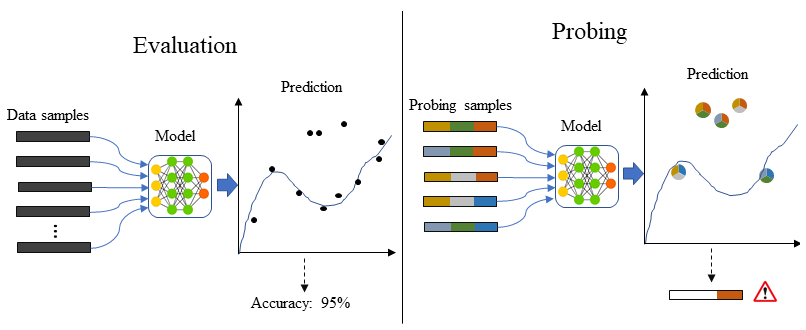
\includegraphics[width=\textwidth]{images/Eva_Prob.png}
\caption{Model evaluation and model probing with controlled data characteristics.}\label{Fig:Prob}
\end{figure}

For this, I examined how two state-of-the-art traffic classifiers could be probed, and performed several experiments to examine the control of DetGen over various traffic characteristics as well as the influence of these traffic characteristics on captured traffic traces with three novel traffic comparison metrics. The results from the probing of the classifiers were prepared into a paper and submitted and accepted at the \textit{Workshop on Traffic Measurements for Cybersecurity}, which is hosted at the \textit{S\&P}-conference in May. The examination of traffic determinism and their impact on traffic traces along with a detailed description of DetGen were submitted as a paper to the 2021 \textit{SecureComm} conference, for which we will receive acceptance notice on 17th May.


\subsection{Short-term contextual model of network flows using LSTM networks}\label{Sec:Short-term}

One of the main strains of work in year 1 and 2 of my PhD was focused on a building a LSTM-based neural network to capture meaningful sequences of \textit{NetFlows} and reflect reccurring patterns in a model. Learned contextual behaviour is reflected through the capability of the model to predict traffic protocols and network ports of flows in a session from a smaller subset of flows, with more accurate predictions being rewarded in the training process.

Despite the promising performance of this model, several submissions a paper to well-known conferences were unsuccessful and the paper was rejected mostly for a lack of novelty and scepticism of the real-world applicability. Last year, this work was finally accepted at the \textit{Machine Learning for Networking}-conference 2020. Some aspects that I improved for acceptance include:

\begin{enumerate}
\item I specified the scope of the model to the detection of U2R and R2L attacks, to which it is more suited than high volume attacks. I also exchanged the evaluation datasets to mutiple ones that are more suitable for this task and more realistic in nature.
\item I extended the model input features and model architecture to capture more complex sequences and decrease areas where the model was not performing well.
\item I replaced the CTU-14-dataset with the more suitable datasets CICIDS-17 and UGR-16, and identified suitable data traces for modelling and analysis. 
\item I focused more on the traffic structures the model is able to detect and explained the corresponding novelty of the model better. 
\item I included several state-of-the-art models as benchmark and also compared the now more complex model to a more shallow version to highlight how the learning of specific traffic structures was improved.
\end{enumerate}


\begin{figure}
\centering
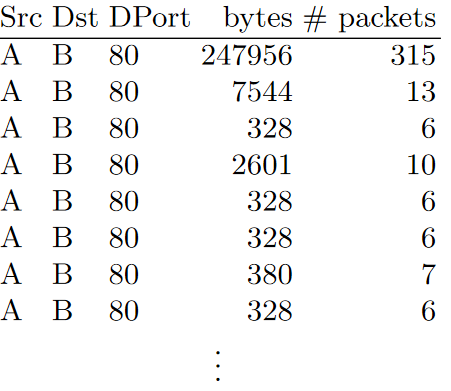
\includegraphics[width=0.4\textwidth]{images/traffic_sequence.png}
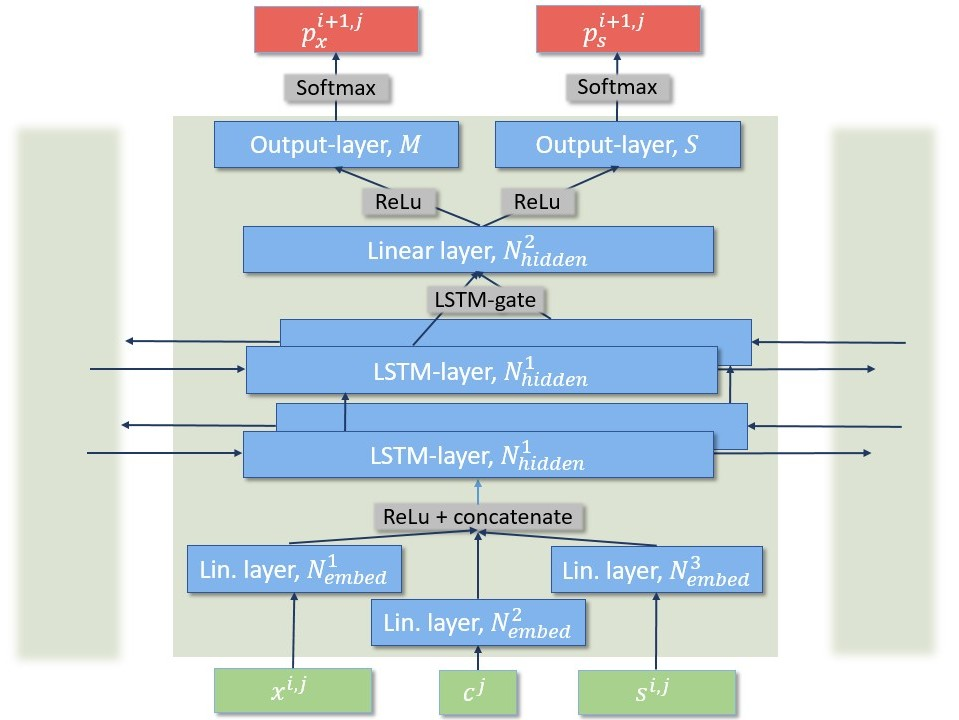
\includegraphics[width=0.49\textwidth]{images/LSTM_design_bi2.jpg}
\caption{Architectures of the model and corresponding traffic sequence of XSS-attack.}
\label{fig:LSTM}
\end{figure}


\subsection{Stepping stone detection}\label{Sec:BTstint}

%As part of my CASE PhD scholarship, I spent six weeks with my industrial sponsor at BT Labs Adastral Park in August and September 2019. Before starting this stint, I met with my industrial supervisors to define a project to work on that is both related to my PhD and is a relevant problem for BT. During this meeting, we agreed that the problem of detecting stepping stones was a suitable topic. 

In a stepping stone scenario, an attacker launches an attack not from their own computer but from intermediary hosts within an enterprise network that were previously compromised, often using an interactive relay session. A common approach in the literature to detect stepping stones is to identify correlation between two connections on a potential intermediary host. Attackers try to evade detection by inserting chaff packets and delays to make the connection appear uncorrelated. %Before starting this 6-week stint, I met with my industrial supervisors where we agreed that the problem of detecting stepping stones is of relevance for them and therefore a suitable topic for my time at BT Labs

The biggest challenge for this problem is that there are no available datasets available that describe stepping stone behaviour. Due to the success of the  DetGen framework, I started to implement several scenarios of interactive traffic relays using SSH-tunnels and netcat/netem for chaff and delay insertion. With this, I was able to generate significant amounts of traffic with a controllable amount of noise and delay to train and assess correlation models.

Since this problem in the described form turned out to not be relevant for BT anymore, I did not proceed to design my own detection method. 
I instead implemented 7 state-of-the-art methods for connection correlation and performed an extensive evaluation of their performance under various circumstances. The corresponding paper was submitted, accepted and published at the \textit{Network and Systems Security} conference 2020.


\begin{figure}
\centering
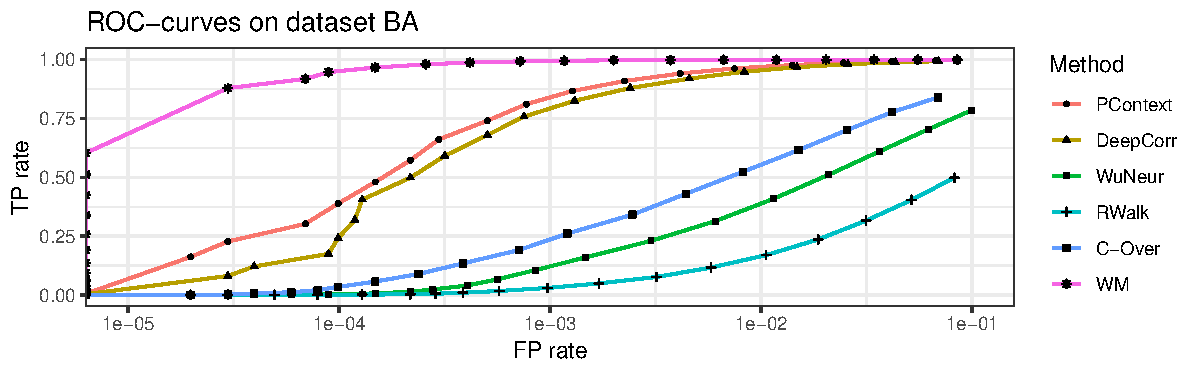
\includegraphics[width=0.9\textwidth]{images/Noevasion_4nodes-1.pdf}
\caption{Evaluation results for methods on the stepping stone data.}\label{stepstone}
\end{figure}

%After more consultation with a security expert, the scope of this project has been altered, which I describe in Section \ref{Bla}

%After finishing the stint at BT Labs, I continued to work on the traffic generation for a bit further before we had a call with Jake Hill, a security expert at BT. This call was meant to provide field knowledge to confirm and/or improve the data generation set-up. However, Jake stated that the problem of attackers launching attacks from intermediary hosts is after all not of great relevance for BT's operations. Instead, his notion of stepping stones described simple proxies relaying services (more on this in Section \ref{Sec:Relay}). In addition, further investigation suggests that the consensus in the literature is that connection correlation produces too many false positives and is not applicable in real-world scenarios. 



\subsection{BT project}\label{Bla}

%As part of my CASE PhD scholarship, I am spending 12 weeks in total with my industrial sponsor at BT Labs Adastral Park in the context of a student placement. While there, I am supposed to conduct research that is both relevant to my PhD-topic and to the operations of BT. Choosing a suitable topic is therefore not completely straightforward and could mean that the research conducted during the placement does not align completely with my PhD-topic.


%In August and September 2019, I spent the first six weeks at Adastral Park. Before starting this stint, I met with my industrial supervisors to define a suitable project to work on. During this meeting, we agreed that the problem of detecting stepping stones was a suitable topic, as it was identified as a pressing issue for BT by their operational team, and could potentially benefit from from the developed DetGen framework described in Section \ref{Sec:BTstint} and the traffic sequence embedding techniques described in Section \ref{Sec:Encoder}.


%After finishing the stint at BT Labs, I continued to work on the traffic generation for a bit further before we had a call with Jake Hill, a security expert at BT. This call was meant to provide field knowledge to confirm and/or improve the data generation set-up. However, Jake stated that the problem of attackers launching attacks from intermediary hosts is after all not of great relevance for BT's operations. 

I am currently involved in a project with BT on the detection of proxies relaying protected content from the perspective of an ISP. Specific characteristics of this problem are:

\begin{itemize}
\item Unlike the original stepping stone problem, these relay proxies operate in a simplistic fashion and do not use evasion tactics. However, content can be forwarded using a different application or protocol than in the first connection.
\item Packets are sampled before observation, meaning that only every n-th packet for each connection is observed.
\item Benign proxies exist that can increase false-positives.
\end{itemize}

Since the start of the project, I have been involved in designing a data generation setup to fit our needs and provide sufficiently challenging data comparable with real-world traffic. I have furthermore examined generated data traces for features and characteristics that we could use in the detection process, and considered multiple potentially suitable detection methods:

\paragraph{Statistical statements about similarity between incoming and outgoing traffic}
By comparing features for both incoming and outgoing traffic on a host during a time window, it might be possible to make statements about unlikely similarity between the two directions. This would again be based on distributions of features like mean observed packets sizes, the number of connections, average transferred bytes, etc. A test on all features could then determine likelihood the two channels being a relay.

\paragraph{Classification-based approaches}
Mining the above described features for a variety of hosts, proxy and non-proxy, and training a robust classifier (logitistic regression, decision tree) on it, such as done in “Detecting Scans at the ISP Level”.

\paragraph{Direct application of Deep-Learning method}
The packet stream on a model could be fed directly into an LSTM model to classify each node. Computationally expensive, but could be used as 2nd step once light indicators are triggered.  However likely to overfit our data.

\begin{figure}
\centering
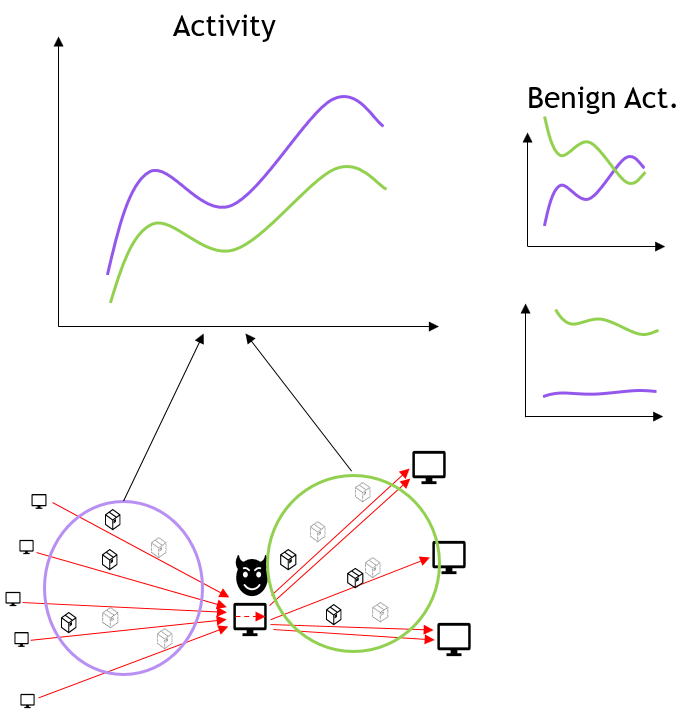
\includegraphics[width=0.6\textwidth]{images/Proxy1.png}
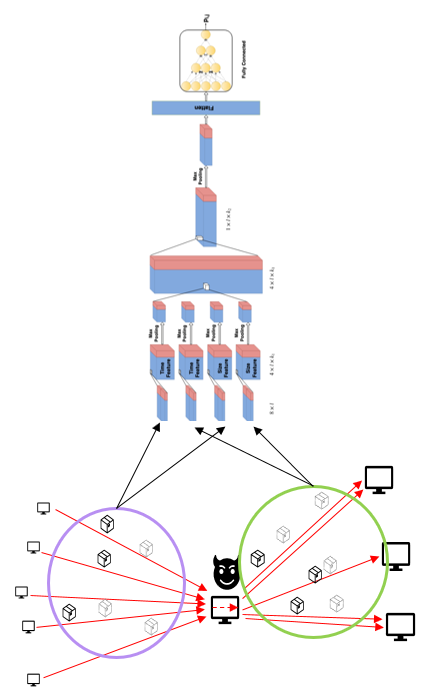
\includegraphics[width=0.38\textwidth]{images/Proxy2}
\caption{Potential methods to detect proxies.}
\label{fig:Proxy}
\end{figure}

At the moment, I am in the process of examining the latest data tranche and will test some of the methods on it. The project recently started moving more quickly, and we will hopefully have a good idea which methods might work in the summer (June/July).

\section{Future plans}

\subsection{QUIC/HTTP examination}

QUIC seeks to improve performance of connection-oriented web-applications using TCP. It is implemented on top of UDP and implements its own TCP-like packet control mechanisms. It allows for multiplexed HTTP-connections and resolves head-of-line blocking during packet loss as well as reducing latency by minimising round-trips during connection establishment. Furthermore, much of the QUIC implementation is moved from kernel to user space, which allows continuous updates of the protocol.

According to an NGINX-spokesperson, "since the protocol is new and things like stack optimization etc. still to catch up and since it's all user-space, there is a possibility to make changes to protocol very rapidly. This generates a higher attack surface than you would have over more layered approach with TCP and http on top." Initial investigations showed that there exists no research on mitigating intrusions over the QUIC protocol.%, which \textcolor{red}{...}

Due to the implementation in user-space, QUIC may introduce vulnerabilities that allow remote code execution on a host, such as in \textit{CVE-2017-15407} and \textit{CVE-2017-15398}. The detection of such code executions by building a combined model of QUIC packet exchanges and process starts/system calls therefore seems like a promising project that provides both novelty and relevance.

In particular, I believe the following conditions would allow for interesting results:
\begin{itemize}
\item Operation on a host (server or client) level
\item Combination of unencrypted packet packet stream and system calls/process starts corresponding
\item A sequential model that applies NLP-techniques to packet content and predicts probability of process start or particular system call (which could then correspond to code execution)
\item Traffic and system call/process log collection using a containerized framework.
\end{itemize}

%One difficulty in this project is that there do not exist many identified vulnerabilities in the QUIC protocol yet, of which none are known to have been used in a successful attack. Therefore, it might be difficult to get enough malicious data for result validation. At this stage of my PhD, beginning a project that is not certain to be successful bears significant risk.  I am therefore currently spending a small amount of time reaching out to experts to verify that data for model validation is available and that the scope of this project is of relevance before fully committing to it.

\subsection{LSTM anomaly detection: Special issue}

After the acceptance and presentation of our LSTM-based anomaly detection model at the MLN conference 2020, we were invited to submit a paper to the \textit{Special Issue ``Selected Papers from the 3rd International Conference on Machine Learning for Networking (MLN'2020)''}. Since over time, a significant amount of material has accumulated that was not included in the MLN-paper, this seems to be a good opportunity to get the remaining work published in this special issue. Specific parts of this material include:
\begin{itemize}
\item Additional details on model operation, likelihood functions, other methods of performing analysis
\item More examination of UGR-content, combined with more analysis of long-term performance
\item UGR-port-scan detection results
\item More extensive comparison with smaller benchmark LSTM-model
\item Results from the LANL dataset
\end{itemize}


\subsection{BT Proxy detection project}
As described above, I am currently investigating data from BT to design appropriate methods to detect proxies in the wild. The goal of this project is to have produced sufficient data, tested methods appropriately, and concluded their reliability and performance by June/July. Depending on the results, this project could produce a joint publication together with BT, who have ambitions to file a corresponding patent.

\section{Publications}

\paragraph{Published:}
\begin{itemize}
\item \textit{Better Anomaly Detection for Access Attacks Using Deep Bidirectional LSTMs}, H Clausen, G Grov, M Sabate, D Aspinall, Machine Learning for Networking: Third International Conference, MLN 2020, Paris, France, November 24–26, 2020,
\item \textit{Evading Stepping-Stone Detection with Enough Chaff}, Clausen, Henry, Michael S. Gibson, and David Aspinall, International Conference on Network and System Security, Melbourne, Australia, November 25-27, 2020
\end{itemize}

\paragraph{Accepted and to be published}
\begin{itemize}
\item \textit{Traffic generation using containerization for machine learning}, Henry Clausen, Robert Flood, David Aspinall, ACSAC DYNAMICS'19: DYnamic and Novel Advances in Machine Learning and Intelligent Cyber Security Workshop in December 09-10, 2019, San Juan, PR
\item \textit{Examining traffic microstructures to improve model development}, Henry Clausen and David Aspinall, Workshop on Traffic Measurements for Cybersecurity at 42th Symposium of Security and Privacy, May 2021, San Francisco
\end{itemize}

\paragraph{Submitted}
\begin{itemize}
\item \textit{Controlling network traffic microstructures for machine-learning model probing}, Henry Clausen, Robert Flood, David Aspinall, SecureComm September 6-9 2021, Canterbury UK
\end{itemize}

\paragraph{Planned}
\begin{itemize}
\item \textit{Additional Material on  Anomaly Detection for Access Attacks Using Deep Bidirectional LSTMs}, Special Issue ``Selected Papers from the 3rd International Conference on Machine Learning for Networking (MLN 2020)'', Deadline: April 30th
\item \textit{Results from proxy detection project}, Appropriate venue not identified yet
\end{itemize}

\section{Thesis structure plan}

\begin{enumerate}
\item \textbf{Central research questions}
\begin{rquestion}\ \\ 
How well-structured is the space of contextual behaviours observed in the traffic of a machine or a network? How much does noise or input variation blur the observable contextual differences between clearly distinct actions?
\end{rquestion}


\begin{rquestion}\ \\
To what degree can contextual structure in network traffic be captured in a model from a training dataset, and how can we achieve this?
\end{rquestion}


\begin{rquestion}\ \\
What is a meaningful representation of traffic structures? What requirements must a labelled traffic generation framework fulfill to provide realistic data?
\end{rquestion}


\begin{rquestion}\ \\
What will a contextual model be able to prevent?
\end{rquestion}


\item \textbf{Background.}
This section gives a general overview over 
 \begin{itemize}
 \item network intrusion detection
 \item anomaly-detection
 \item network traffic
 \end{itemize}

\item \textbf{Design and requirements on semantic anomaly-detection models.}
This section acts as a motivation on 
 \begin{itemize}
 \item what the design of a semantic anomaly-detection model can potentially identify, i.e. anomalous packet or flow sequences that are a results of specific exploits. 
 \item what model design could capture corresponding structures for the detection
 \end{itemize}

This section would furthermore discuss 

\begin{itemize}
 \item why microstructures in the traffic are necessary to be leveraged by such a model
 \item what influence different factors could have on these structures and corresponding models
 \end{itemize}



\item \textbf{Flow-level semantic anomaly-model and structures it can learn/detect}.
This section will contain the majority of the MLN LSTM-paper and the additional material on applications to the LANL data. It will highlight
 \begin{itemize}
 \item What structures can be observed on a flow level
 \item which attacks affect structures on a flow-level, and in what way
\item how our model is able learn flow-level structures and identify these deviations
\item what steps were necessary in terms of model expansion to learn complex structures
 \end{itemize}

\item \textbf{Packet-level semantic encoder and how it internalises traffic structures}.
I am not sure whether to include this section. It would contain the work I made to build an encoder-decoder model of packet sequences. I did not perform any anomaly-detection with it, but it could give very interesting insights into how a model internalises packet-sequence structures due to the latent-space projection inherent to this model.

\item \textbf{Quantifying effect of factors on microstructures.}
This section would contain most of the work conducted in the SecureComm-paper, i.e.
 \begin{itemize}
 \item the proposal and explanation of traffic similarity metrics
 \item measurement and analysis of the influence of different factors (congestion, implementations, activities, etc.)
 \end{itemize}

\item \textbf{Examining the effect of microstructure perturbations on model performance.}
This section would contain most of the work conducted in the WTMC-paper, i.e.
 \begin{itemize}
 \item two examples on how models are affected by traffic influence factors
 \end{itemize}

\item \textbf{Effect of adversarial microstructure perturbations on stepping-stone detection}
This section would contain the results of the stepping-stone paper, but
 \begin{itemize}
 \item focus on the perturbations
 \item why specific models (DeepCorr, PContext) are not able to identify learned structures anymore when facing sufficient perturbations
 \end{itemize}
 

\item \textbf{Controlling influence on traffic microstructures.}
This section would contain the setup of DetGen and the corresponding experimental verifications of its determinism.




\end{enumerate}


%In the light of the problems described in Section \ref{Sec:Problems} that we encountered in the field of anomaly-based intrusion detection, I believe that the scope of this PhD-project has to be altered slightly. As there will not be enough material directly concerning anomaly detection, the formulation of building anomaly-detection models describing software behaviour should be relaxed to general applications of ML (not just anomaly detection) in specific areas related to software defined behaviour. 
%The overall unifying theme of this PhD so far has been centered around small-scale traffic structures generated by software-defined computer interactions and applications of ML language models to it, in other words \textbf{Modelling computer interactions as a language}.
%This could be based of the reoccurring use of traffic (and potentially system/program logs) generation for machine learning. The generated traffic could then be verified as valuable by the implemented intrusion detection applications.

%All applications implemented so far except for the flow-level model are driven (in part) by our traffic generation:
%\end{itemize}
\subsection{Thesis Completion plan}

\begin{itemize}


\item April
\begin{itemize}
\item Collate LSTM-materials into a paper and submit to special issue on 30th April deadline
\item Finish section 2 and 3 (background and detection requirements) of the thesis
\item Implement simple benchmark methods on proxy-data
\item Discuss final scope of QUIC/HTTP-project
\item Potential work on the QUIC/HTTP-project
\end{itemize}

\item May
\begin{itemize}
\item Extend and test proxy detection methods on larger background data
\item Finish section 4 and 5 (both on anomaly models) of the thesis
\item Potential work on QUIC/HTTP-project
\end{itemize}

\item June
\begin{itemize}
\item Finish section 6 and 7 (WTMC and SecureComm-papers) of the thesis
\item Present proxy detection results at the Stats and Cyber Security Session at JSM 2021 (were I was invited to speak)
\item Revise literature review
\item Potential work on QUIC/HTTP-project
\end{itemize}

\item July
\begin{itemize}
\item Finish proxy-detection work, hopefully with a well-performing model as the result
\item Discuss potential publication of the proxy-detection results
\item Finish section 8, 9, and 1 of the thesis
\item Potential work on the QUIC/HTTP-project
\end{itemize}

\item August
\begin{itemize}
\item Revise thesis and add potential additional examinations (models, traffic)
\item Potential work on the QUIC/HTTP-project
\item Potentially write paper on proxy-detection work (needs permission from BT-supervisors)
\end{itemize}

\item September
\begin{itemize}
\item Revise and submit thesis
\item Prepare for viva
\end{itemize}

\end{itemize}

\section{Impact of COVID-19 on progression}

The closure of the PhD-offices in the Informatics forum and the work-from-home directive lead to a less productive work environment at home with significantly more distractions. Roughly I am 1-2 hours less productive every day. I also had to invest a significant amount of time rearranging the work situation appropriately.
Face-to-face meetings over Skype have been helpful and easy to set up, but it is more difficult to go through paper drafts or discuss work  in detail. 
Overall, I had significantly less contact and conversations with people who could potentially have valuable input and stimulating thoughts, loss of opportunity to network at international conferences.
Internet speed has had a minor impact on data availability.


%\addcontentsline{toc}{section}{Bibliography}
%\bibliographystyle{abbrv}
%\bibliography{refs}

\end{document}